\documentclass{standalone}
\usepackage{tikz}
\usetikzlibrary{decorations.pathreplacing,decorations.pathmorphing}
\usetikzlibrary{fit,quotes}
\usepackage{yquant, braket}

\begin{document}
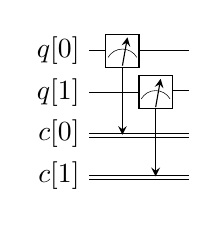
\begin{tikzpicture}[scale=1.000000,x=1pt,y=1pt]
\filldraw[color=white] (0.000000, -7.500000) rectangle (36.000000, 52.500000);
% Drawing wires
% Line 1: q0 W q[0]
\draw[color=black] (0.000000,45.000000) -- (12.000000,45.000000);
%\draw[color=black] (12.000000,44.500000) -- (36.000000,44.500000);
\draw[color=black] (12.000000,45.00000) -- (36.000000,45.00000);
\draw[color=black] (0.000000,45.000000) node[left] {$q[0]$};
% Line 2: q1 W q[1]
\draw[color=black] (0.000000,30.000000) -- (24.000000,30.000000);
%\draw[color=black] (24.000000,29.500000) -- (36.000000,29.500000);
\draw[color=black] (24.000000,30.500000) -- (36.000000,30.500000);
\draw[color=black] (0.000000,30.000000) node[left] {$q[1]$};
% Line 3: c0 W c[0]
\draw[color=black] (0.000000,15.000000) -- (36.000000,15.000000);
\draw[color=black] (0.000000,15.000000) node[left] {$c[0]$};
\draw[color=black] (0.000000,13.5000000) -- (36.000000,13.5000000);
% Line 4: c1 W c[1]
\draw[color=black] (0.000000,0.000000) -- (36.000000,0.000000);
\draw[color=black] (0.000000,0.000000) node[left] {$c[1]$};
% Done with wires; drawing gates
% Line 5: q0:cwire +c0
%\draw (11.500000,45.000000) -- (11.500000,15.000000);
\draw (12.00000,45.000000) -- (12.00000,25.000000);
\filldraw (12.000000, 45.000000) circle(1.500000pt);
\begin{scope}
%\draw[fill=white] (12.000000, 15.000000) circle(3.000000pt);
\clip (12.000000, 15.000000) circle(3.000000pt);
\draw (9.000000, 15.000000) -- (15.000000, 15.000000);
%\draw (12.000000, 12.000000) -- (12.000000, 18.000000);
\end{scope}
\draw[fill=white] (6.000000, 39.000000) rectangle (18.000000, 51.000000);
\draw[very thin] (12.000000, 45.600000) arc (90:150:6.000000pt);
\draw[very thin] (12.000000, 45.600000) arc (90:30:6.000000pt);
\draw[->,>=stealth] (12.000000, 39.600000) -- +(80:10.392305pt);
% Line 6: q1:cwire +c1
%\draw (23.500000,30.000000) -- (23.500000,0.000000);
\draw (24.00000,30.000000) -- (24.00000,0.000000);
\filldraw (24.000000, 30.000000) circle(1.500000pt);
\begin{scope}
%\draw[fill=white] (24.000000, 0.000000) circle(3.000000pt);
\clip (24.000000, 0.000000) circle(3.000000pt);
\draw (21.000000, 0.000000) -- (27.000000, 0.000000);
%\draw (24.000000, -3.000000) -- (24.000000, 3.000000);
\end{scope}
\draw[fill=white] (18.000000, 24.000000) rectangle (30.000000, 36.000000);
\draw[very thin] (24.000000, 30.600000) arc (90:150:6.000000pt);
\draw[very thin] (24.000000, 30.600000) arc (90:30:6.000000pt);
\draw[->,>=stealth] (24.000000, 24.600000) -- +(80:10.392305pt);
\draw[->,>=stealth] (24.000000, 10.00000)  -- +(270:10.392305pt); % arrowhead
\draw[->,>=stealth] (12.000000, 25.00000)  -- +(270:10.392305pt); % arrowhead
\draw[color=black] (0.000000,-1.5000000) -- (36.000000,-1.5000000);
%\draw (42.000000, 25.00000) node[text width=144pt,below,text centered] {\scriptsize or};
% Done with gates; drawing ending labels
% Done with ending labels; drawing cut lines and comments
% Done with comments
\end{tikzpicture}
\end{document}
